\documentclass{beamer} % imports amsmath symbols

\usepackage{mathleague}

\newcommand{\contestproblemset}{12117}
\newcommand{\roundname}{Target}
\newcommand{\problemnumber}{4}

\begin{document}

\begin{frame} % Title Page
  \titlepage
\end{frame}

\section{Problem Statement}

\subsection*{Identify our objective.}

\begin{frame}
An equiangular but not equilateral hexagon has three times the area of a regular hexagon with side length $1$. If both hexagons have whole number side lengths, then what is the perimeter of the larger hexagon?
\end{frame}

\section{Solution}

\subsection*{Find the perimeter of an equiangular (non-equilateral) hexagon that has thrice the area of a regular hexagon with side length $1$.}

\begin{frame}
  \begin{center}
    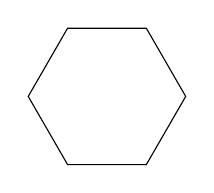
\begin{tikzpicture}
      \draw (0,0) -- (-0.5,0.866025404) -- (0,1.73205081) -- (1,1.73205081) -- (1.5,0.866025404) -- (1,0) -- cycle;
    \end{tikzpicture}
  \end{center}
\end{frame}

\begin{frame}
  \begin{center}
    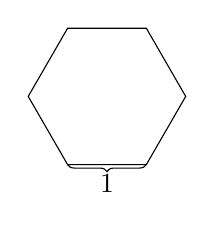
\begin{tikzpicture}
      \draw (0,0) -- (-0.5,0.866025404) -- (0,1.73205081) -- (1,1.73205081) -- (1.5,0.866025404) -- (1,0) -- cycle;
      \draw [decoration={brace,mirror,raise=0cm},decorate] (0,0) -- (1,0) node [midway,below=0.0cm] {$1$};
    \end{tikzpicture}
  \end{center}
\end{frame}

\begin{frame}
  \begin{center}
    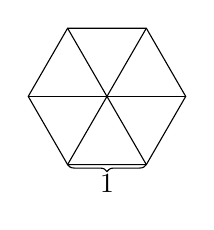
\begin{tikzpicture}
      \draw (0,0) -- (-0.5,0.866025404) -- (0,1.73205081) -- (1,1.73205081) -- (1.5,0.866025404) -- (1,0) -- cycle;
      \draw (0,0) -- (0.5,0.866025404);
      \draw (-0.5,0.866025404) -- (0.5,0.866025404);
      \draw (0,1.73205081) -- (0.5,0.866025404);
      \draw (1,1.73205081) -- (0.5,0.866025404);
      \draw (1.5,0.866025404) -- (0.5,0.866025404);
      \draw (1,0) -- (0.5,0.866025404);
      \draw [decoration={brace,mirror,raise=0cm},decorate] (0,0) -- (1,0) node [midway,below=0.0cm] {$1$};
    \end{tikzpicture}
    
    \pause
    Area of a regular hexagon with side length $1$
    \[
    = 6 \cdot \frac{1}{2} \cdot 1 \cdot \frac{\sqrt{3}}{2}\pause = \frac{3}{2} \cdot \sqrt{3}
    \]
  \end{center}
\end{frame}

\begin{frame}
  \begin{center}
    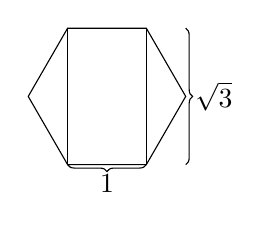
\begin{tikzpicture}
      \draw (0,0) -- (-0.5,0.866025404) -- (0,1.73205081) -- (1,1.73205081) -- (1.5,0.866025404) -- (1,0) -- cycle;
      \draw (0,0) -- (0,1.73205081);
      \draw (1,0) -- (1,1.73205081);
      \draw [decoration={brace,mirror,raise=0.5cm},decorate] (1,0) -- (1,1.73205081) node [midway,right=0.5cm] {$\sqrt{3}$};
      \draw [decoration={brace,mirror,raise=0.0cm},decorate] (0,0) -- (1,0) node [midway,below=0.0cm] {$1$};
    \end{tikzpicture}
  \end{center}
\end{frame}

\begin{frame}
  \begin{center}
    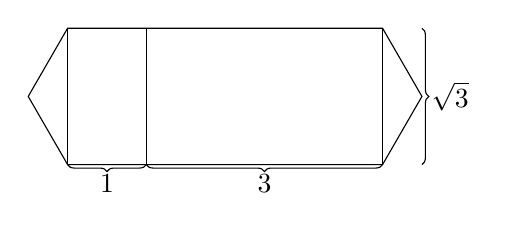
\begin{tikzpicture}
      \draw (0,0) -- (-0.5,0.866025404) -- (0,1.73205081) -- (4,1.73205081) -- (4.5,0.866025404) -- (4,0) -- cycle;
      \draw (0,0) -- (0,1.73205081);
      \draw (1,0) -- (1,1.73205081);
      \draw (4,0) -- (4,1.73205081);
      \draw [decoration={brace,mirror,raise=0.5cm},decorate] (4,0) -- (4,1.73205081) node [midway,right=0.5cm] {$\sqrt{3}$};
      \draw [decoration={brace,mirror,raise=0.0cm},decorate] (0,0) -- (1,0) node [midway,below=0.0cm] {$1$};
      \draw [decoration={brace,mirror,raise=0.0cm},decorate] (1,0) -- (4,0) node [midway,below=0.0cm] {$3$};
    \end{tikzpicture}
  \end{center}
\end{frame}

\begin{comment}
    \begin{tikzpicture}[scale=0.5]
      %\draw (0,4.46971821313) node [above left] {$A$};
      %\draw (0,0) node [below left] {$B$};
      %\draw (14.3185760149,0) node [right] {$C$};
      \draw (0,0) -- (0,4.46971821313);
      \draw (0,0) -- (14.3185760149,0);
      \draw (0,4.46971821313) -- (14.3185760149,0) node [midway,above] {$15$};
      \coordinate (A) at (0,4.46971821313);
      \coordinate (B) at (0,0);
      \coordinate (C) at (14.3185760149,0);
      \tkzMarkRightAngle(A,B,C)
    \end{tikzpicture}
\end{comment}

\setcounter{equation}{0}

\section{Conclusion}

\subsection*{Review the key concepts we used.}

\begin{frame}{Key Concepts}
  \pause
  \begin{itemize}
  \item Area of an Equilateral Triangle
  \pause
  \item Area of a Regular Hexagon
  \end{itemize}
\end{frame}

\end{document}